\chapter{Introduction}

\section{Physics and detector context}

The Compressed Baryonic Matter (CBM) experiment at FAIR is designed to study strongly interacting matter at high net-baryon density under laboratory conditions \citep{Friman2011CBMPhysicsBook}. Within that program, reliable event characterization is essential: centrality determination, reaction-plane reconstruction, and the interpretation of event-by-event observables all depend on a robust measurement of forward-going spectator matter. The forward detector system therefore has a direct impact on the quality of the physics extracted from heavy-ion data, especially in the high-rate environment foreseen for CBM.

The Forward Spectator Detector (FSD) has been developed as the dedicated forward detector for spectator nucleons and nuclear fragments in CBM. Its role is to provide event-plane information and support centrality reconstruction at the interaction rates relevant for the experiment \citep{Dvorak2025FSD}. However, charged spectators alone do not provide the full picture of the forward final state. A measurement of neutral forward particles, especially neutrons, is required if the forward system is to deliver a more complete description of spectator emission and its correlation with the collision geometry.

The Neutron Calorimeter (NCAL) addresses this missing neutral component. According to the current NCAL addendum, the detector is intended to complement the FSD by measuring forward neutral spectators and thereby strengthening centrality and collective-flow related measurements in the CBM heavy-ion program \citep{Okropiridze2026NCALAddendum}. The same document also emphasizes a broader physics reach: forward neutron detection can support dedicated studies of elementary channels such as proton-proton and deuteron-proton reactions, and may provide a handle for initial-state neutron tagging in deuteron-induced interactions \citep{Okropiridze2026NCALAddendum}. In that sense, NCAL is not merely an auxiliary subsystem, but a detector with its own performance questions and physics potential.

The present NCAL prototype program is built around repurposed detector components originating from the COSY Time-of-Flight system, combined into dedicated test configurations for commissioning and performance studies \citep{Okropiridze2024SimulationNCAL,Okropiridze2026NCALAddendum}. Prototype setups have been used both in the mini-CBM environment at GSI and in external test campaigns, including measurements at \NCALInstitute \citep{Okropiridze2026NCALAddendum}. These campaigns are scientifically important because they provide controlled conditions under which detector response can be studied before the final integration of NCAL into the CBM forward system.

\section{Motivation for the present study}

The main objective of the present work is to characterize the NCAL prototype at a level that is useful for detector development, future integration, and later publication. In practical terms, this means quantifying how the detector responds in a neutron-beam environment, identifying which observables carry the strongest discriminating power, and determining which aspects of the readout chain are stable enough to support reproducible analysis.

One central question is the neutron detection efficiency of the detector under the beam conditions available during the test campaign. That quantity is directly relevant for evaluating whether the prototype geometry, active material, and readout concept are adequate for the role envisioned for NCAL in the CBM forward system. Efficiency, however, is not the only quantity of interest. A useful neutron detector must also be understood in terms of timing behavior, prompt backgrounds, and event-selection quality. For that reason, the present study also treats particle-identification methods as a core topic rather than a secondary analysis exercise.

The detector-development aspect of this work is equally important. The campaign is not only a neutron-response measurement; it is also a test bench for readout and data-acquisition concepts. In particular, the study is intended to improve the understanding of NCAL performance when operated with the newly developed DOGMA front-end electronics and with the older DiRICH-based chain used in earlier detector work. Even when the final CBM readout choice lies outside the scope of this document, comparative operation with these chains is highly informative because it exposes differences in timing reference quality, signal handling, data integrity, and downstream analysis requirements. A careful comparison is therefore part of understanding the detector itself. The second campaign at \NCALInstitute should therefore be understood primarily as a detector-characterization and readout-validation experiment rather than as a finalized production-data run.

\subsection{Motivation from the first campaign at \NCALInstitute}

The present campaign should be read explicitly as experiment~2. According to the current run history, the preceding campaign used a proton-on-lithium neutron-production target in a fixed-position configuration. In that first experiment, the gamma-induced population formed a broad structure directly beneath the neutron-candidate region in the time-of-flight versus pulse-height plane. Under those conditions, the overlap between the two populations made it very difficult to characterize the NCAL detector response cleanly.

Figure~\ref{fig:rez1-gamma-neutron-overlap} documents that limitation using the time-of-flight-overlay version of the first-campaign plot. The figure is included here because it captures the central practical reason for carrying out a second campaign under modified conditions: the dominant lower population and the neutron-candidate accumulation were not sufficiently separated in the observable space available in experiment~1. For comparison, the same figure also includes an analytical estimate of the prompt-gamma and \SI{30}{MeV} neutron time-of-flight dependence on detector distance, together with the corresponding time-of-flight difference.

\begin{figure}[tbp]
\centering
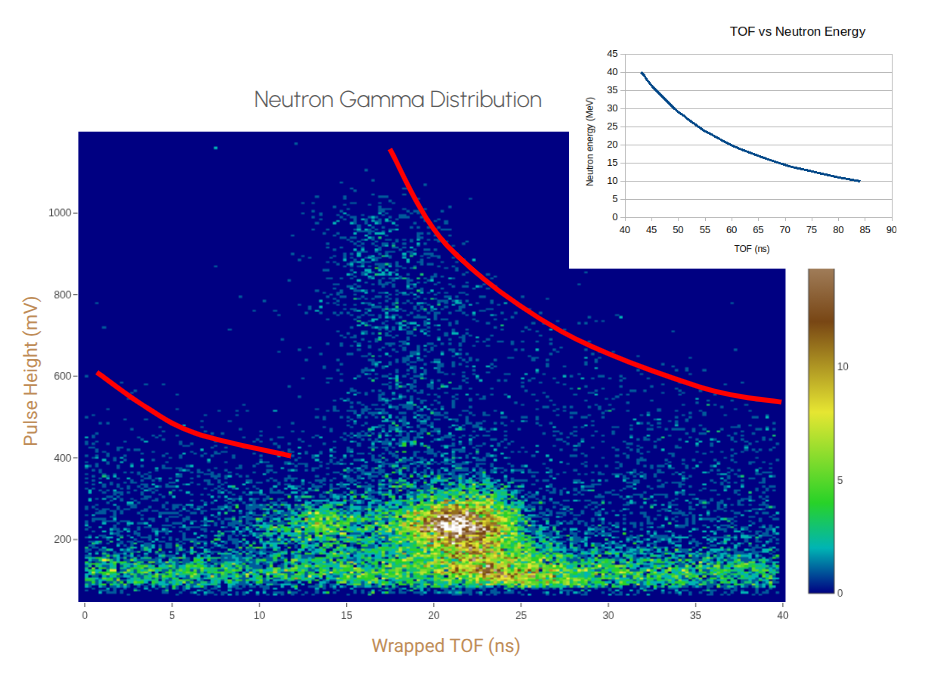
\includegraphics[width=0.88\textwidth,height=0.34\textheight,keepaspectratio]{figures/NCAL_Gamma_NEutron_hist_REZ1_TOFoverlay.png}

\vspace{0.8em}

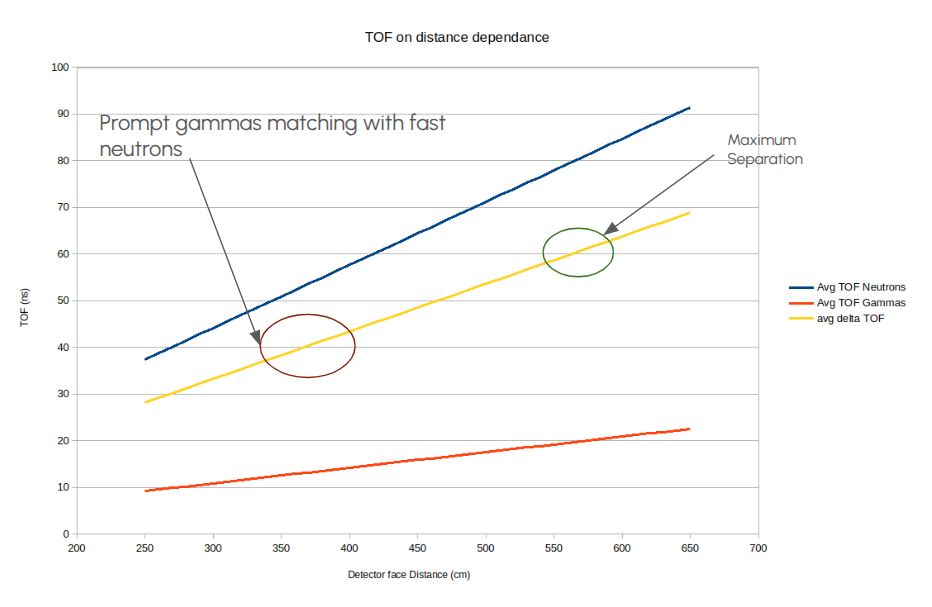
\includegraphics[width=0.88\textwidth,height=0.34\textheight,keepaspectratio]{figures/Gamma_Neutron_deltaTOF_30MeVneutrons.png}
\caption{Top: wrapped time-of-flight versus pulse-height distribution from the first campaign at \NCALInstitute, shown in the time-of-flight-overlay form used during later interpretation of the dataset. In the working interpretation of experiment~1, the broad lower population corresponds to gamma-induced events, while the higher-time-of-flight structure contains the neutron-candidate region. Bottom: analytical estimate of prompt-gamma time of flight, \SI{30}{MeV} neutron time of flight, and the corresponding time-of-flight difference as a function of detector-face distance. Together, the two panels illustrate why limited timing separation in the first campaign made a clean characterization of the NCAL response difficult.}
\label{fig:rez1-gamma-neutron-overlap}
\end{figure}

\section{Scope of this document}

This document is being developed as a broad scientific record of the second experimental campaign and is intended to mature into material suitable for a thesis chapter and, after further refinement, parts of one or more journal articles. Its purpose is therefore twofold. First, it should document the experiment rigorously enough that the measurement logic, detector configuration, and analysis choices remain transparent and reproducible. Second, it should separate verified results from working hypotheses, so that later interpretation can be strengthened without rewriting the experimental history.

The analysis workflow already points toward the structure needed for such a document. The existing event-digestion tools extract trigger-referenced observables such as leading and trailing edge times, time-over-threshold values, trigger-to-trigger spacing, and timing jitter from raw DOGMA-formatted data. These observables are natural building blocks for beam-structure studies, time-of-flight analysis, and future particle-identification strategies. Accordingly, the full document should evolve toward a coherent treatment of the experimental setup, beam conditions, detector geometry, veto configuration where applicable, DAQ architecture, calibration logic, event reconstruction, uncertainty sources, and performance observables.

At the present stage, the introduction is intentionally conservative. It establishes the detector and physics context from available project documents and defines the immediate scientific aims of this campaign: characterization of NCAL, evaluation of neutron-response observables, exploration of PID strategies, and assessment of detector operation together with DOGMA and DiRICH readout concepts. Subsequent chapters can build on this foundation by adding the finalized beamline description, analysis methodology, efficiency extraction strategy, uncertainty treatment, and validated experimental results.